\documentclass[12pt]{article}
\usepackage{caption}
\usepackage{graphicx, subfig}
\usepackage{float}
\usepackage{mathptmx}
\usepackage{graphicx}
\usepackage{listings}
\usepackage{amsmath}
\usepackage{amssymb}
\usepackage{algorithm}
\usepackage{color}

\definecolor{dkgreen}{rgb}{0,0.6,0}
\definecolor{gray}{rgb}{0.5,0.5,0.5}
\definecolor{mauve}{rgb}{0.58,0,0.82}

\lstset{frame=tb,
  language=Python,
  aboveskip=3mm,
  belowskip=3mm,
  showstringspaces=false,
  columns=flexible,
  basicstyle={\small\ttfamily},
  numbers=none,
  numberstyle=\tiny\color{gray},
  keywordstyle=\color{blue},
  commentstyle=\color{dkgreen},
  stringstyle=\color{mauve},
  breaklines=true,
  breakatwhitespace=true,
  tabsize=3
}
\title{HenriquezHHtest}
\author{Student Name: Fanjie Kong
\\
Student ID: 2462691 }

\begin{document}
\maketitle
\newpage
\textbf{Result:}
\\\\
Starting simulation at t=0. s for a duration of 5. ms\\
0.005 (100\%) simulated in $<$ 1s
\\
Starting simulation at t=5. ms for a duration of 1. ms\\
0.001 (100\%) simulated in $<$ 1s 
\\
Starting simulation at t=0. s for a duration of 5. ms\\
0.005 (100\%) simulated in $<$ 1s
\\
Starting simulation at t=5. ms for a duration of 1. ms\\
0.001 (100\%) simulated in $<$ 1s
\\

Process finished with exit code 0
\\
 \begin{figure}[H]
  \centering
  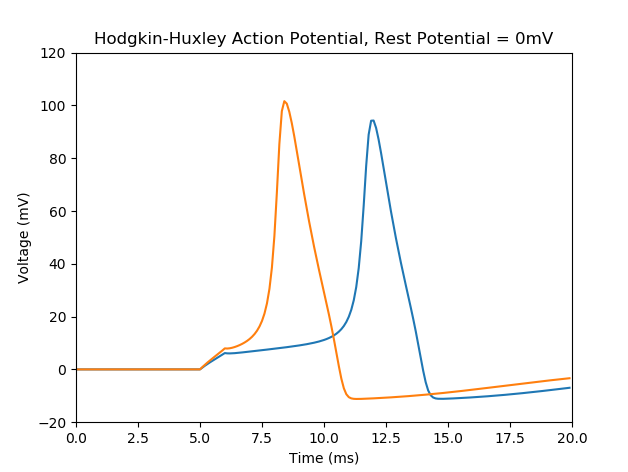
\includegraphics[width=.8\textwidth]{h1_p1.png} %1.png是图片文件的相对路径
  \label{img} %此处的label相当于一个图片的专属标志,目的是方便上下文的引用
  \caption{Result}
\end{figure}
\end{document}